%
% $RCSfile: singleton.tex,v $
%
% Copyright (c) 2004. Christian Heller. All rights reserved.
%
% No copying, altering, distribution or any other actions concerning this
% document, except after explicit permission by the author!
% At some later point in time, this document is planned to be put under
% the GNU FDL license. For now, _everything_ is _restricted_ by the author.
%
% http://www.cybop.net
% - Cybernetics Oriented Programming -
%
% http://www.resmedicinae.org
% - Information in Medicine -
%
% @author Christian Heller <christian.heller@tuxtax.de>
%

\paragraph{Singleton}
\label{singleton_heading}

Whenever an object-oriented system wants to ensure that only one instance of a
certain class exists, the \emph{Singleton} pattern \cite{gamma1995} can be used.
It essentially is a class which encapsulates its instance's data and provides
global access to them, via \emph{static}, sometimes called \emph{class} methods
(figure \ref{singleton_figure}).\\

A \emph{Registry} object as described by Fowler \cite{fowler2002} often uses the
\emph{Singleton} pattern, to be unique and to become globally accessible.
Similarly do many so-called \emph{Manager} objects, for example change managers
which are also responsible for the caching of objects.

Global, that is static access -- the main purpose of the \emph{Singleton} pattern,
is its main weakness, at the same time (section \ref{global_access_heading}). One
obvious solution to avoid singleton objects could be to forward global information
from component to component, possibly using an own \emph{Lifecycle Method}, as
described in Apache Jakarta's \emph{Avalon Framework} \cite{avalon}. This approach,
however, might bring with a rather large number of parameters to be handed over.
The search for further alternatives therefore remains a topic of interest.

\begin{figure}[ht]
    \begin{center}
        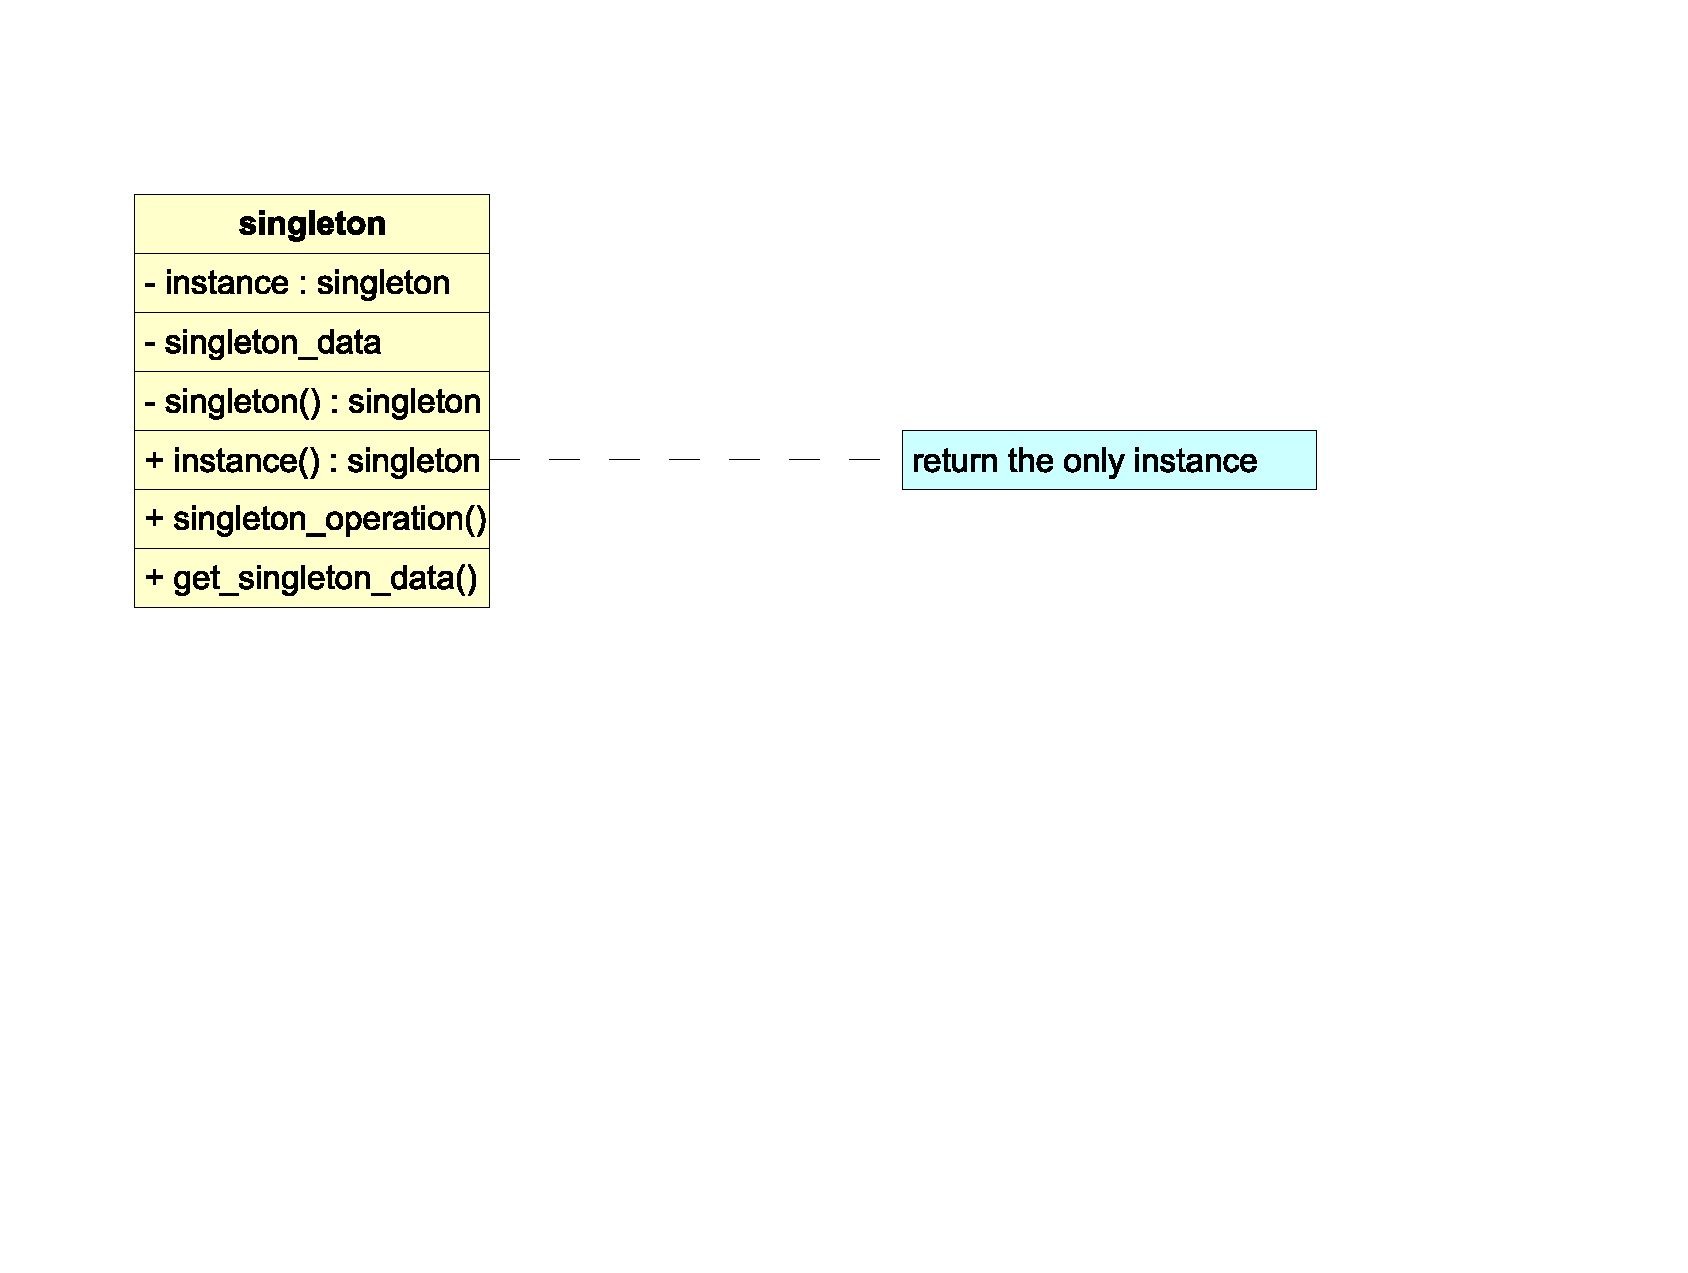
\includegraphics[scale=0.3]{vector/singleton.eps}
        \caption{Singleton Pattern}
        \label{singleton_figure}
    \end{center}
\end{figure}
